\documentclass[11pt]{article}
\usepackage[a4paper,margin=25mm]{geometry}
\usepackage[T1]{fontenc}
\usepackage{lmodern,microtype,amsmath,amssymb,amsthm,mathtools}
\usepackage{graphicx,booktabs,array,enumitem,xcolor,xurl}
\emergencystretch=1em
\usepackage[colorlinks=true,linkcolor=blue!45!black,citecolor=blue!45!black,urlcolor=blue!45!black]{hyperref}
\usepackage[capitalise,noabbrev]{cleveref}
\hypersetup{pdfauthor={Shivam Gupta},pdftitle={Which Complex Poles Are Compatible with Unresolved Data?}}
\usepackage{fancyhdr}
\setlength{\headheight}{14pt}
\pagestyle{fancy}\fancyhf{}\fancyhead[L]{\small Heat-structured pole reachability}\fancyhead[R]{\small S. Gupta}\fancyfoot[C]{\thepage}
\setlength{\parskip}{3pt}\setlength{\parindent}{1.2em}
\newtheorem{theorem}{Theorem}\newtheorem{proposition}[theorem]{Proposition}\newtheorem{corollary}[theorem]{Corollary}\newtheorem{lemma}[theorem]{Lemma}\theoremstyle{remark}\newtheorem{remark}[theorem]{Remark}
\newcommand{\R}{\mathbb R}\newcommand{\C}{\mathbb C}\newcommand{\T}{\mathbb T}\newcommand{\norm}[1]{\left\lVert #1\right\rVert}\newcommand{\range}{\operatorname{range}}
\title{Which Complex Poles Are Compatible with Unresolved Data?\\[3pt]\large Sharp Sobolev-Tail Bounds for Periodic Burgers Flow}
\author{Shivam Gupta\\\small Independent Researcher\\\small\href{mailto:shivam1720406@gmail.com}{shivam1720406@gmail.com}}
\date{17 October 2026}
\begin{document}
\maketitle
\begin{abstract}
Complex singularities provide useful diagnostics of nonlinear evolution, but a pole inferred from resolved data need not be stable under unresolved modes. We study this distinction for periodic viscous Burgers flow by perturbing its normalized Cole--Hopf potential in a real Sobolev ball while fixing its resolved Fourier coefficients. The heat semigroup maps that ball to an explicitly computable ellipse at each complex point. Its inverse image gives the exact minimum initial-tail norm required to place a pole there, together with an attaining perturbation. A positivity condition ensures that every admissible perturbation defines a real, globally regular Burgers solution. We obtain an exact shared-budget criterion for several requested zeros, a contour certificate preserving zero counts, and a sharp small-time asymptotic whose exponential factor is $\exp[-y^2/(4\nu t)]$. For a single-cosine center we characterize the worst-case analyticity width exactly. At $\nu t=0.02$, a nominal width of $0.725915\ldots$ falls to a rigorously bracketed robust width in $(0.5816,0.5817)$ under an $H^1$ tail budget of $0.01$. Two individually attainable poles require over four times the larger individual budget when imposed together. Reproducible software supplies outward-rounded infinite-tail bounds, 31 width brackets, ten contour certificates, independent interpolation checks, and a forward Burgers computation. The results specialize classical pseudozero and minimum-norm interpolation ideas to physically admissible unresolved heat data.
\end{abstract}
\noindent\textbf{Keywords:} complex singularities; viscous Burgers equation; Cole--Hopf transformation; pseudozeros; Sobolev uncertainty; validated numerics.\\
\noindent\textbf{Code and computational records:}\\
\noindent\url{https://github.com/shi1720/heat-pole-reachability}.

\section{Introduction}
A complex pole can encode information about the steepness and spectral resolution of a real solution without producing a singularity on the physical domain. This makes singularity tracking an attractive diagnostic. It also creates a question that a nominal pole plot cannot answer: which singularities are consequences of the resolved data, and which depend on an unresolved tail?

This paper answers that question for a specific, analytically tractable model. Consider $2\pi$-periodic viscous Burgers flow,
\begin{equation}\label{eq:burgers}
 u_t+uu_x=\nu u_{xx},\qquad \nu>0.
\end{equation}
The Cole--Hopf representation writes $u=-2\nu\partial_x\log\phi$, where $\phi_t=\nu\phi_{xx}$. We fix the mean of $\phi$ to one. A strictly positive real initial potential yields a real, regular solution for positive time; complex zeros of the evolved potential yield poles of its logarithmic derivative.

Our data model fixes the Fourier coefficients of the initial potential through mode $N$ and bounds the remaining real coefficients in a Sobolev norm. The question is then a worst-case one over a specified deterministic uncertainty set. It is neither an estimate from a random-noise model nor a claim that low modes of the velocity determine low modes of its Cole--Hopf potential.

A simple example makes the issue quantitative. Let the center be $p_0(x)=1+0.8\cos x$. At scaled time $\tau=\nu t=0.02$, its closest complex zeros are at $\pi\pm0.725915\ldots i$. Fix its mean and first mode, and allow an unresolved tail with norm
\[
 \norm{h}_1^2=\sum_{k=2}^{\infty}k^2(a_k^2+b_k^2)\le 10^{-4}.
\]
Every admissible initial potential remains positive. Nevertheless, an explicit tail of norm $0.0085523\ldots$ creates a pole at $\pi+0.59i$. The largest strip guaranteed pole-free for \emph{every} tail in the ball has half-width between $0.5816$ and $0.5817$. A nominal continuation therefore answers a materially different question from a robust one.

The contribution has four parts. First, we give an exact, constructive distance-to-pole formula that retains the real structure of the initial data. Second, we characterize simultaneous pole requests under one common tail, rather than combining pointwise possibilities as if they were independent. Third, we derive a sharp small-time law and an exact robust-width characterization for the single-cosine family. Fourth, we provide a continuous-contour verification procedure with explicit infinite-series bounds and reproducible computations. The underlying Hilbert-space interpolation and pseudozero principles are classical; the specific object here is the uncertainty in Burgers singularities induced by unresolved positive real heat data.

\section{Related work and scope of the contribution}
The Cole--Hopf linearization is due to Hopf and Cole \cite{hopf,cole}. Spectral diagnosis of complex singularities has a substantial history, including Sulem, Sulem, and Frisch \cite{sulem} and Weideman \cite{weideman}. VandenHeuvel et al. \cite{vandenheuvel} combine exact representations, asymptotics, and AAA approximation to examine Burgers poles. Lustri et al. \cite{lustri} develop exponential-asymptotic and transseries descriptions. Gentner, Dallaston, and McCue \cite{gentner} investigate singularities generated by piecewise-continuous initial conditions. These works motivate the diagnostic, but do not formulate the Sobolev-tail uncertainty set studied here.

Rational approximation is an effective tool for numerical analytic continuation; the AAA algorithm \cite{aaa} and Trefethen's survey \cite{continuation} provide relevant foundations. The ill-conditioning of continuation itself is well established \cite{illconditioning}. Our results do not make that inverse problem well conditioned. They replace one nominal continuation by an exact statement about a declared family of continuations.

Pseudozero sets describe the zeros of nearby functions, most commonly polynomials. Graillat and Langlois \cite{pseudozeros} distinguish real from complex polynomial perturbations and give computable descriptions. Our real evaluation ellipse is a heat-weighted infinite-dimensional instance of this principle, not a new general pseudozero theory. Likewise, the common-tail Gram formula is minimum-norm interpolation in a real Hilbert space, consistent with reproducing-kernel theory \cite{aronszajn}. Connections between heat reachability and spaces of analytic functions have been developed in different settings, including boundary-controlled finite rods \cite{lopez} and general domains \cite{strohmaier}. Here ``reachability'' means placing specified \emph{complex zeros} by changing bounded initial Fourier tails; it does not mean boundary controllability of the heat equation.

\begin{table}[t]
\centering\small
\caption{The mathematical question isolated in this paper. These are distinctions of scope, not performance rankings.}\label{tab:position}
\begin{tabular}{@{}>{\raggedright\arraybackslash}p{.27\linewidth}>{\raggedright\arraybackslash}p{.31\linewidth}>{\raggedright\arraybackslash}p{.35\linewidth}@{}}\toprule
Established framework & Main object & Object studied here\\\midrule
Burgers singularity tracking & Poles of a specified solution & Poles compatible with a fixed resolved spectrum and bounded tail\\
Polynomial pseudozeros & Roots under coefficient perturbations & Real Sobolev perturbations propagated by the heat semigroup\\
Minimum-norm interpolation & Least-norm function meeting linear conditions & Shared initial data producing several zeros or prescribed zero multiplicity\\
Validated numerics & Rigorous arithmetic and enclosures & Continuous-contour exclusion for an infinite admissible family\\\bottomrule
\end{tabular}
\end{table}

The contribution boundary matters. We do not introduce the Cole--Hopf transform, real pseudozeros, Gram interpolation, or ball arithmetic. We supply an explicit positivity-compatible specialization, its sharp time asymptotic and robust-width consequence, and a checked implementation. The references above identify the closest foundations located in our review.

\section{An uncertainty class with positive real initial data}
Let $s>1/2$ and $N\ge0$ be an integer. A real tail has the form
\begin{equation}\label{eq:tail}
 h(x)=\sum_{k>N}(a_k\cos kx+b_k\sin kx),\qquad
 \norm{h}_s^2=\sum_{k>N}k^{2s}(a_k^2+b_k^2).
\end{equation}
This norm convention is fixed throughout; for $s=1$ it equals $\pi^{-1}\int_0^{2\pi}|h'(x)|^2\,dx$. The absence of low modes includes the mean. A periodic positive potential describes zero-mean velocities; a known nonzero mean can be removed by a Galilean shift. Let $p_0$ be a real trigonometric polynomial of mean one, with $p_0(x)\ge m>0$. Its degree need not equal $N$. Define
\begin{equation}\label{eq:uncertainty}
 \mathcal A_{N,s}(\eta)=\{p_0+h:\norm{h}_s\le\eta\},\qquad
 B_{N,s}=\left(\sum_{k>N}k^{-2s}\right)^{1/2}.
\end{equation}
Every member has the same coefficients as $p_0$ through mode $N$.

\begin{lemma}[Uniform positivity]\label{lem:positivity}
If $\eta B_{N,s}<m$, every member of $\mathcal A_{N,s}(\eta)$ is continuous and strictly positive on $\T$. Its heat evolution remains positive on the real axis. Its Cole--Hopf velocity solves \eqref{eq:burgers} classically for $t>0$.
\end{lemma}
\begin{proof}
At each real $x$, Cauchy--Schwarz and $\cos^2kx+\sin^2kx=1$ give $|h(x)|\le\norm{h}_s B_{N,s}$. The same estimate on tails establishes uniform convergence. Hence $p_0+h\ge m-\eta B_{N,s}>0$. Positivity follows under the periodic heat semigroup, and differentiation of its logarithm gives the Burgers equation. Heat smoothing makes the solution classical for positive time.
\end{proof}

Write $\tau=\nu t$ and
\begin{equation}\label{eq:heat}
 H_\tau h(z)=\sum_{k>N}e^{-\tau k^2}(a_k\cos kz+b_k\sin kz),\quad
 \phi_h(z,\tau)=p(z,\tau)+H_\tau h(z),
\end{equation}
where $p=H_\tau p_0$. For $\tau>0$, these series and all spatial derivatives converge locally uniformly in $\C$ by Gaussian decay. Thus $\phi_h$ is entire and periodic. It is not identically zero since its mean is one. A zero of multiplicity $q$ at $z_*$ produces
\begin{equation}\label{eq:residue}
 u_h(z,t)=-\frac{2\nu q}{z-z_*}+O(1).
\end{equation}
The pole is simple as a meromorphic singularity, even when the zero has multiplicity greater than one. When preserving a count below, we count potential zeros \emph{with multiplicity}; equivalently we preserve the sum of pole residues divided by $-2\nu$.

\section{An exact distance to a compatible pole}
For $y\ne0$, define the positive, convergent sums
\begin{align}
 C_{N,s}(y,\tau)&=\sum_{k>N}k^{-2s}e^{-2\tau k^2}\cosh^2(ky),\label{eq:C}\\
 S_{N,s}(y,\tau)&=\sum_{k>N}k^{-2s}e^{-2\tau k^2}\sinh^2(ky).\label{eq:S}
\end{align}
They are even in $y$, with $C>S>0$. Suppress subscripts when unambiguous.

\begin{theorem}[Exact real-tail radius]\label{thm:radius}
At $z=x+iy$, $y\ne0$, the minimum of $\norm{h}_s$ subject to $\phi_h(z,\tau)=0$ is
\begin{equation}\label{eq:radius}
 r_{N,s}(z,\tau)^2=
 \frac{(\Re p(z,\tau))^2}{C_{N,s}(y,\tau)}+
 \frac{(\Im p(z,\tau))^2}{S_{N,s}(y,\tau)}.
\end{equation}
The minimum is attained. In particular, a zero is compatible with the closed ball of radius $\eta$ if and only if $r_{N,s}(z,\tau)\le\eta$. Under \cref{lem:positivity}, this is also exact compatibility with a physically admissible positive initial potential in the stated class.
\end{theorem}
\begin{proof}
Rotate the two real coefficients at each mode by
\[
 A_k=a_k\cos kx+b_k\sin kx,\qquad
 D_k=-a_k\sin kx+b_k\cos kx.
\]
The rotation preserves $a_k^2+b_k^2$. With $d_k=e^{-\tau k^2}$,
\[
 H_\tau h(x+iy)=\sum_{k>N}d_k A_k\cosh ky
       +i\sum_{k>N}d_k D_k\sinh ky.
\]
The real and imaginary evaluation functionals act on orthogonal coefficient subspaces. Their squared dual norms are $C$ and $S$. Let $v_R=-\Re p(z,\tau)$, $v_I=-\Im p(z,\tau)$. Cauchy--Schwarz gives the lower bound $\norm{h}_s^2\ge v_R^2/C+v_I^2/S$. Equality holds for
\begin{equation}\label{eq:witness}
 A_k=\frac{v_R d_k\cosh ky}{Ck^{2s}},\qquad
 D_k=\frac{v_I d_k\sinh ky}{Sk^{2s}},
\end{equation}
followed by the inverse rotation. These sequences belong to the coefficient Hilbert space and satisfy the two constraints. This also handles $p(z,\tau)=0$, when $h=0$ is optimal.
\end{proof}

The image of the norm ball under evaluation is precisely the filled ellipse with semiaxes $\eta\sqrt C$ and $\eta\sqrt S$. A circular majorant encloses it in the disk of radius $\eta\sqrt C$. That relaxation yields the sufficient exclusion test $|p|>\eta\sqrt C$, while \eqref{eq:radius} uses both components exactly. Its radius is at least the circular-test radius $|p|/\sqrt C$. Equality holds for real $p$; strict gains require an imaginary component. We do not claim a universal improvement in strip width from the ellipse: the symmetric family in \cref{sec:width} attains its worst case where $p$ is real, so the two tests agree there.

At $y=0$, the imaginary evaluation vanishes. The corresponding unconstrained interpolation radius is $|p(x,\tau)|/\sqrt{C(0,\tau)}$. Under the positivity condition this cannot be attained within the admissible budget. The apparent degeneracy $S=0$ is therefore a real-structure constraint, not a numerical singularity to be removed by complexifying the data.

\begin{figure}[t]
\centering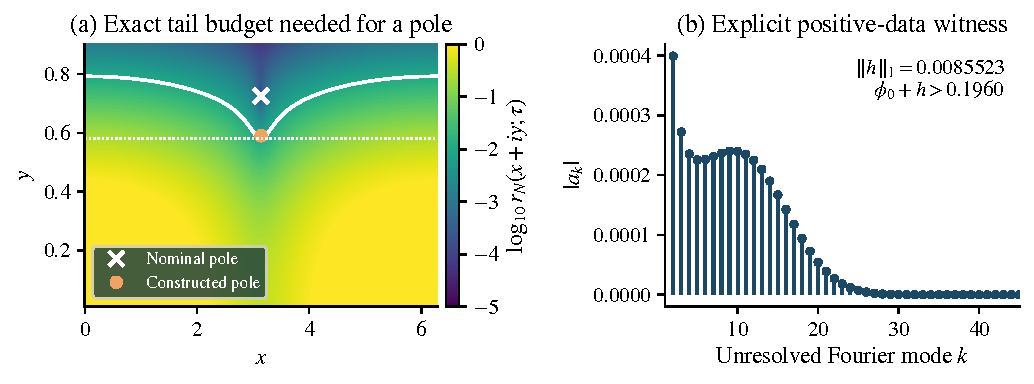
\includegraphics[width=\linewidth]{../figures/reachability.pdf}
\caption{An exact uncertainty diagnostic for $p_0=1+0.8\cos x$, $N=s=1$, $\tau=0.02$. Left: the minimum tail norm needed to place a pole at each point; the white contour is $r=0.01$. The dotted line marks the verified pole-free height $0.5816$. Right: coefficients of a finite witness placing a pole at $\pi+0.59i$, with norm below $0.01$ and strictly positive initial potential. The rasterized color field is illustrative; the reported width bounds use ball arithmetic.}\label{fig:map}
\end{figure}

\section{Several poles must share one initial tail}
Pointwise membership in a pseudozero set does not mean that several points can be zeros of the same member. This distinction is essential when interpreting a collection of candidate poles.

Normalize coefficients as $\theta_{k,c}=k^sa_k$, $\theta_{k,s}=k^sb_k$. For a point $z$ and nonnegative derivative order $j$, define the complex coefficient row
\begin{equation}\label{eq:row}
 e_{z,j}(k,c)=e^{-\tau k^2}k^{j-s}\cos(kz+j\pi/2),\quad
 e_{z,j}(k,s)=e^{-\tau k^2}k^{j-s}\sin(kz+j\pi/2).
\end{equation}
Taking real and imaginary parts of these rows produces a bounded real operator $L:\ell^2(\R)\to\R^d$ for any finite list of constraints. Let $v$ stack the corresponding values $-\Re\partial_z^jp$ and $-\Im\partial_z^jp$, and let $G=LL^*$.

\begin{theorem}[Shared-tail interpolation]\label{thm:joint}
The constraints $L\theta=v$ are attainable if and only if $v\in\range G$. When attainable, the exact minimum squared norm is
\begin{equation}\label{eq:joint}
 r_{\mathrm{joint}}^2=v^\top G^\dagger v,\qquad
 \theta_*=L^*G^\dagger v.
\end{equation}
Thus they are compatible with the radius-$\eta$ ball if and only if $v\in\range G$ and $v^\top G^\dagger v\le\eta^2$. Requiring $j=0,\ldots,q-1$ at a point imposes a zero of multiplicity at least $q$.
\end{theorem}
\begin{proof}
A finite-rank operator has $\range L=\range(LL^*)$ and closed range. If $v$ lies in that range, $L\theta_*=GG^\dagger v=v$. The vector $\theta_*$ lies in $\range L^*$ and is orthogonal to $\ker L$. Every feasible vector is $\theta_*+w$, $w\in\ker L$, so Pythagoras establishes optimality and the stated squared norm. If $v$ is outside the range, the constraints are inconsistent. The derivative statement follows from the definition of zero multiplicity.
\end{proof}

This is the classical minimum-norm interpolation calculation. Its role here is to encode that \emph{one} real initial tail must explain every requested singularity. Conjugate points impose redundant constraints, since $\phi_h(\bar z)=\overline{\phi_h(z)}$. They must not be treated as independent pole requests. The pseudoinverse formulation retains this redundancy; the numerical implementation uses a rank-revealing SVD for finite exploratory problems.

For $x=\pi$ and a single-cosine center, the real constraints at positive heights $y_i$ reduce to
\[
 G_{ij}=\sum_{k>N}\frac{e^{-2\tau k^2}\cosh(ky_i)\cosh(ky_j)}{k^{2s}},\qquad
 v_i=-\bigl(1+\alpha e^{-\tau}\cosh(y_i)\cos\pi\bigr).
\]
At $\tau=0.02$, $N=s=1$, $\alpha=0.8$, heights $0.58$ and $0.60$ require individual norms $0.0102964\ldots$ and $0.00704220\ldots$. Their simultaneous minimum is $0.0416299\ldots$. With $\eta=0.02$, each is possible separately, but they cannot coexist. All these budgets satisfy the uniform positivity condition; the incompatibility is not caused by allowing nonphysical initial data.

\begin{figure}[t]
\centering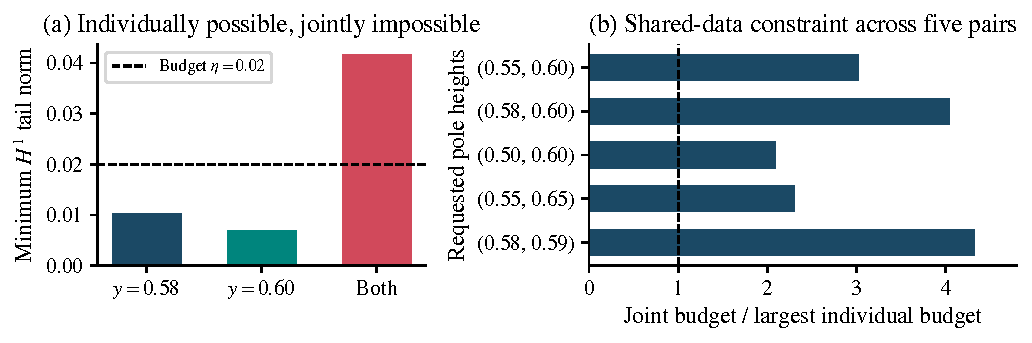
\includegraphics[width=\linewidth]{../figures/joint.pdf}
\caption{Pointwise compatibility does not imply joint compatibility. Both poles in the left panel are individually possible within the dashed budget, but their shared-tail minimum exceeds it. Right: the joint norm divided by the larger individual norm for five height pairs. The computations include the infinite tail in the Gram enclosures.}\label{fig:joint}
\end{figure}

\section{Small-time loss of robust complex information}
The heat semigroup damps real high frequencies, but evaluation off the real axis multiplies a mode by a hyperbolic factor. Their competition selects a moving band of unresolved modes.

\begin{theorem}[Sharp fixed-height small-time law]\label{thm:asymptotic}
Fix $s>1/2$, a finite $N$, and $y>0$. As $\tau\downarrow0$,
\begin{equation}\label{eq:saddle}
 C_{N,s}(y,\tau)\sim S_{N,s}(y,\tau)
 \sim\frac14\left(\frac{y}{2\tau}\right)^{-2s}
 \sqrt{\frac{\pi}{2\tau}}\exp\left(\frac{y^2}{2\tau}\right).
\end{equation}
If $p_0(x+iy)\ne0$, then
\begin{equation}\label{eq:asymptotic}
 r_{N,s}(x+iy,\tau)\sim
 2|p_0(x+iy)|\left(\frac{y}{2\tau}\right)^s
 \left(\frac{2\tau}{\pi}\right)^{1/4}
 \exp\left(-\frac{y^2}{4\tau}\right).
\end{equation}
\end{theorem}
\begin{proof}
Expand $\cosh^2ky=(e^{2ky}+2+e^{-2ky})/4$ and $\sinh^2ky=(e^{2ky}-2+e^{-2ky})/4$. The dominant sum in both cases is one quarter of
\[
 \sum_{k>N}k^{-2s}\exp(-2\tau k^2+2ky)
 =e^{y^2/(2\tau)}\sum_{k>N}k^{-2s}e^{-2\tau(k-k_*)^2},\quad k_*=\frac{y}{2\tau}.
\]
In the window $|k-k_*|\le\tau^{-3/4}$, $k/k_*=1+O(\tau^{1/4})$, uniformly, so $k^{-2s}=k_*^{-2s}(1+o(1))$. The Gaussian lattice sum is asymptotic to $\sqrt{\pi/(2\tau)}$ by a rescaled Riemann sum. Outside that window, Gaussian decay is exponentially small relative to the central sum: splitting additionally at $k=k_*/2$ bounds the polynomial factor uniformly in the upper portion, while the finitely weighted lower portion is exponentially suppressed. Removing the fixed modes through $N$ does not change the leading term. The sums from $2$ and $e^{-2ky}$ remain bounded because $\sum k^{-2s}<\infty$, and are negligible relative to the dominant exponential. This proves \eqref{eq:saddle}. Since $p(z,\tau)\to p_0(z)$ and $C\sim S$, substitution in \eqref{eq:radius} gives \eqref{eq:asymptotic}.
\end{proof}

\begin{corollary}[Positive-data ambiguity at any fixed height]\label{cor:ambiguity}
Fix a finite $N$, $y>0$, $x\in\R$, and a positive budget satisfying $\eta B_{N,s}<m$. At all sufficiently small positive times, a member of $\mathcal A_{N,s}(\eta)$ has a pole at $x+iy$. The attaining initial tail may depend on time.
\end{corollary}
\begin{proof}
If $p_0(x+iy)\ne0$, \cref{thm:asymptotic} gives $r\to0$. If $p_0(x+iy)=0$, $p(x+iy,\tau)$ remains bounded while both $C$ and $S$ diverge, giving the same conclusion directly from \eqref{eq:radius}. Positivity holds uniformly by \cref{lem:positivity}.
\end{proof}

This statement concerns robustness across an uncertainty class. It does not assert that one fixed perturbation develops a pole at every requested point, nor that the real solution blows up. The active mode is approximately $k_*=y/(2\tau)$; increasing a fixed resolution modestly can leave this band essentially untouched. This predicts a practical limitation of interpreting early-time complex poles from a short spectrum.

\begin{figure}[t]
\centering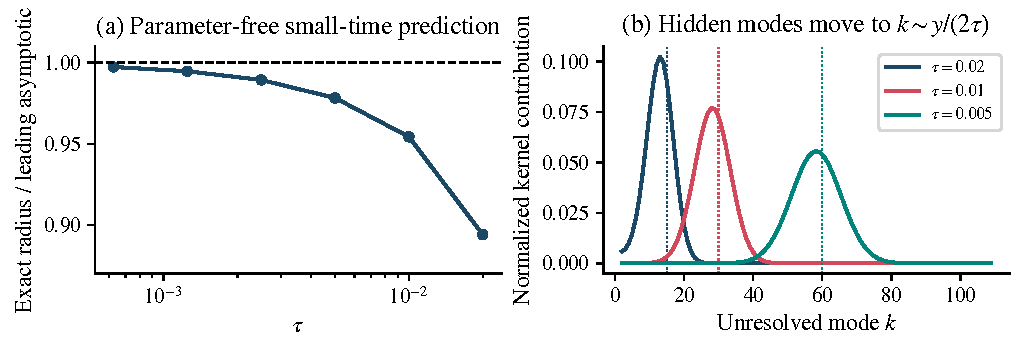
\includegraphics[width=\linewidth]{../figures/asymptotics.pdf}
\caption{Small-time mechanism at $z=2+0.6i$, $N=s=1$. Left: exact radius divided by the leading expression using $p(z,\tau)$ in place of $p_0(z)$ to isolate the kernel asymptotic. No exponent is fitted. The ratio increases from $0.8940$ at $\tau=0.02$ to $0.9974$ at $\tau=0.000625$. Right: normalized dominant summands and the predicted saddle locations (dotted).}\label{fig:asymptotic}
\end{figure}

\section{Exact robust widths and a resolution criterion}\label{sec:width}
For a general center, a robust analyticity strip can be certified by excluding zeros throughout it, or by a zero-free boundary homotopy and a nominal zero count. A single-cosine center permits an exact reduction without spatial optimization.

\begin{theorem}[Sharp width for a single-cosine center]\label{thm:width}
Let $p_0(x)=1+\alpha\cos x$, $0<\alpha<1$, and assume $\eta B_{N,s}<1-\alpha$. Put $A=\alpha e^{-\tau}$ and $y_0=\operatorname{arcosh}(1/A)$. There is a unique $Y_\eta\in(0,y_0)$ satisfying
\begin{equation}\label{eq:width}
 \frac{1-A\cosh Y_\eta}{\sqrt{C_{N,s}(Y_\eta,\tau)}}=\eta.
\end{equation}
Every admissible solution is pole-free for $|\Im z|<Y_\eta$. A member has a pole at $\pi+iY_\eta$, so this open-strip half-width is optimal for the uncertainty class.
\end{theorem}
\begin{proof}
For $|y|\le Y<y_0$, $\Re p(x+iy,\tau)=1+A\cos x\cosh y\ge1-A\cosh Y>0$. Since $C(y,\tau)$ increases with $|y|$, \eqref{eq:radius} yields
\[
 r_{N,s}(x+iy,\tau)\ge\frac{1-A\cosh Y}{\sqrt{C(Y,\tau)}}.
\]
Equality holds at $x=\pi$, $y=Y$. The right side is continuous and strictly decreasing on $[0,y_0]$, ending at zero. At $Y=0$, $\sqrt{C(0,\tau)}\le B_{N,s}$, so its value exceeds $\eta$ by the assumed positivity bound. The unique crossing gives \eqref{eq:width}; \cref{thm:radius} supplies the attaining tail. Any larger open strip contains that pole.
\end{proof}

\begin{proposition}[A sufficient resolution test]\label{prop:resolution}
Let $s=1$, $L=N+1$, $Y\ge0$, and $\rho=\exp[-2\tau(2L+1)+2Y]<1$. Then
\begin{equation}\label{eq:resolution}
 C_{N,1}(Y,\tau)\le
 Q_N(Y,\tau):=\frac{L^{-2}\exp(-2\tau L^2+2YL)}{1-\rho}.
\end{equation}
If $|p|\ge d>0$ on a contour contained in $|\Im z|\le Y$ and $\eta\sqrt{Q_N}<d$, every admissible potential has the nominal zero count inside that contour.
\end{proposition}
\begin{proof}
Each summand of $C$ is at most $q_k=k^{-2}e^{-2\tau k^2+2Yk}$. For $k\ge L$, its consecutive ratios are at most $\rho$. Summation gives \eqref{eq:resolution}. The circular enclosure then ensures $|H_\tau h|<|p|$ on the contour, and Rouch\'e's theorem applies.
\end{proof}

The proposition is sufficient and can be conservative. The exact radius remains the principal diagnostic. It provides a computable stopping criterion for resolving additional modes, once a valid tail norm bound and a contour margin are available. It does not estimate that norm from a truncated spectrum.

\begin{figure}[t]
\centering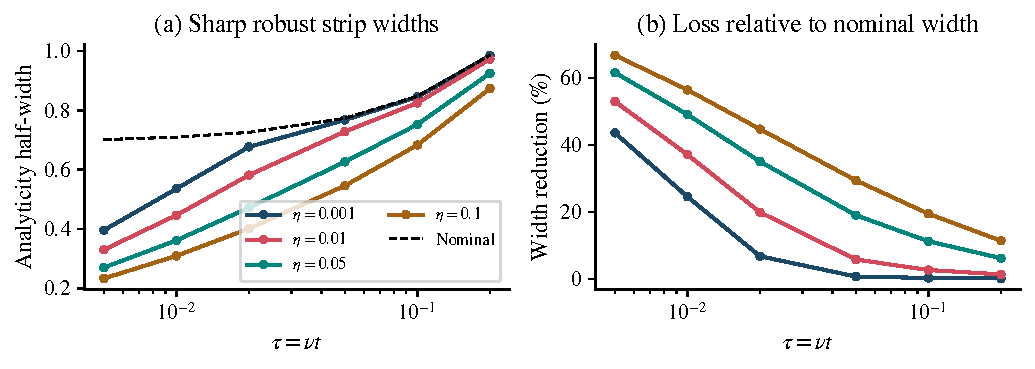
\includegraphics[width=\linewidth]{../figures/widths.pdf}
\caption{Sharp robust widths for $p_0=1+0.8\cos x$, $N=s=1$. All 24 plotted cases have outward-rounded brackets of width $10^{-4}$. The nominal width is shown dashed. The right panel reports its relative reduction under the same uncertainty sets.}\label{fig:widths}
\end{figure}

\section{Continuous certificates and computational method}
\subsection{Zero-count preservation}
\begin{proposition}[Real-structure contour certificate]\label{prop:contour}
Let $\Gamma$ be a positively oriented simple closed piecewise-smooth contour and $\tau>0$. If $r_{N,s}(z,\tau)>\eta$ at every nonreal point of $\Gamma$ and real-axis points are excluded by positivity, then all $\phi_h$, $\norm{h}_s\le\eta$, have the same number of zeros inside $\Gamma$, counted with multiplicity.
\end{proposition}
\begin{proof}
For any such $h$, the family $p+\lambda H_\tau h$, $0\le\lambda\le1$, lies in the same uncertainty ball. The radius condition and positivity exclude a zero on $\Gamma$ throughout the homotopy. The argument principle makes the integer zero count invariant. This conclusion requires a continuous contour condition; checking only sampled nodes is insufficient.
\end{proof}

\subsection{Infinite tails and interval subdivision}
The reference implementation, called HeatTail, separates floating-point exploration from outward-rounded certification. The latter uses FLINT/Arb \cite{arb} at 160-bit precision. Rational center coefficients are entered as exact rational strings. Decimal parameter strings are enclosed by Arb; exploratory binary coordinates used to select a contour are subsequently treated as those exact binary inputs.

For $s=1$, summing \eqref{eq:C}--\eqref{eq:S} through $K$ leaves a nonnegative tail in either sum bounded by
\begin{equation}\label{eq:tailbound}
 T_K=\frac{(K+1)^{-2}\exp[-2\tau(K+1)^2+2Y(K+1)]}
 {1-\exp[-2\tau(2K+3)+2Y]},
\end{equation}
provided the denominator is positive. This is the same geometric estimate as \cref{prop:resolution}, now applied after a finite sum. Increasing $K$ tightens the enclosure; no unresolved coefficients are silently set to zero. The main certificates use $K=300$, and the resolution sweep uses $K=400$.

For each line segment of a rectangular contour, the code encloses $p$ on a complex interval box covering the entire segment. It combines lower bounds for $|\Re p|$ and $|\Im p|$ with upper bounds for $C$ and $S$ to obtain a lower bound on $r$. A box is accepted only when that bound exceeds $\eta$ and its nominal image excludes zero. Otherwise it is bisected. Reaching the depth limit produces an unresolved result, never a successful certificate.

An accepted interval image is convex and excludes zero, so the nominal curve on that segment is homotopic to its endpoint chord without crossing zero. Outward-rounded principal argument increments of the endpoint ratios therefore determine the winding of the nominal image. The code also checks that each increment has magnitude strictly below $\pi$. It accepts the total only when its enclosure identifies one integer winding number. Together with \cref{prop:contour}, this is a certificate for the whole uncertainty family. A reversed contour has the opposite winding; the mathematical zero count uses positive orientation.

For a full rectangular zero-free region, the companion routine recursively bounds $r$ on its interior boxes. The single-cosine width results also have the independent analytic reduction in \cref{thm:width}. For upper width bounds, a finite-mode version of \eqref{eq:witness} supplies an exact interpolation witness with an enclosed norm below $\eta$. Its coefficients are defined by the formula, not by rounding the saved plotting array. A plot or a small floating residual alone is not used as a proof of a zero.

\section{Reproducible computational results}
\subsection{Design and reported quantities}
All experiments use deterministic parameter lists or recorded pseudorandom seeds. There is no training set and no fitted asymptotic exponent. The repository contains source, tests, machine-readable parameters and results, plotting code, and the manuscript source. Floating exploratory values, interval certificates, and analytic deductions have separate roles.

The main center is $p_0=1+0.8\cos x$, with $s=N=1$. We evaluate six scaled times $\tau\in\{0.005,0.01,0.02,0.05,0.1,0.2\}$ and four budgets $\eta\in\{0.001,0.01,0.05,0.1\}$. Since $B_{1,1}=\sqrt{\pi^2/6-1}$, even the largest ball satisfies $p_0+h\ge0.1196\ldots>0$. Each of the 24 width cases has a lower zero-free bound and an upper witness bound separated by $10^{-4}$. Seven additional resolution cases have brackets no wider than $10^{-6}$.

\begin{table}[t]
\centering\small
\caption{Selected sharp robust-width brackets, $N=s=1$. Each interval is established by an exclusion below and a constructive witness above; displayed endpoints are conservative decimal values.}\label{tab:widths}
\begin{tabular}{@{}rrrrr@{}}\toprule
$\tau$ & Nominal width & $\eta=0.001$ & $\eta=0.01$ & $\eta=0.1$\\\midrule
0.005 & 0.701444 & (0.3956, 0.3957) & (0.3298, 0.3299) & (0.2329, 0.2330)\\
0.010 & 0.709669 & (0.5356, 0.5357) & (0.4464, 0.4465) & (0.3090, 0.3091)\\
0.020 & 0.725915 & (0.6768, 0.6769) & (0.5816, 0.5817) & (0.4012, 0.4013)\\
0.050 & 0.773174 & (0.7677, 0.7678) & (0.7284, 0.7285) & (0.5457, 0.5458)\\
0.100 & 0.847834 & (0.8454, 0.8455) & (0.8252, 0.8253) & (0.6829, 0.6830)\\
0.200 & 0.985978 & (0.9846, 0.9847) & (0.9727, 0.9728) & (0.8738, 0.8739)\\\bottomrule
\end{tabular}
\end{table}

\subsection{Resolution and joint compatibility}
At $\tau=0.005$, $\eta=0.01$, fixing additional modes increases the guaranteed width as shown in \cref{tab:resolution}. Increasing $N$ from 1 to 16 changes it by less than $0.001$, whereas resolving through mode 128 nearly restores the nominal width. This behavior agrees with the moving high-frequency band in \cref{thm:asymptotic}; the observation is conditional on the same residual norm budget at each resolution.

\begin{table}[t]
\centering\small
\caption{Resolution sensitivity at $\tau=0.005$, $\eta=0.01$, $s=1$. Values are rounded exploratory roots backed by stored brackets of width at most $10^{-6}$; the nominal width is $0.701443923\ldots$.}\label{tab:resolution}
\begin{tabular}{@{}rrrrrrr@{}}\toprule
$N$ & 1 & 16 & 32 & 64 & 96 & 128\\\midrule
$Y_\eta$ & 0.329802 & 0.330664 & 0.343522 & 0.432043 & 0.557553 & 0.686068\\\bottomrule
\end{tabular}\\[4pt]
At $N=160$, $0.701443<Y_\eta<0.701444$.
\end{table}

Five pairs of heights test the distinction between separate and simultaneous feasibility. Their joint-to-largest-individual norm ratios range from $2.09$ to $4.32$ (\cref{fig:joint}). These are exact interpolation comparisons for prescribed points, not a statistical estimate of the prevalence of incompatible pole sets.

\subsection{Asymmetric centers and continuous contours}
To avoid restricting contour verification to an even, single-mode center, we also use
\begin{align*}
 p_{0,2}(x)&=1+\tfrac12\cos x+\tfrac3{20}\cos2x+\tfrac2{25}\sin2x,\\
 p_{0,3}(x)&=1+\tfrac25\cos x+\tfrac1{20}\sin x+\tfrac1{10}\cos2x
             -\tfrac2{25}\sin2x+\tfrac1{20}\cos3x+\tfrac3{100}\sin3x.
\end{align*}
Their elementary positivity lower bounds are $0.33$ and $0.410515\ldots$. We fix modes through $N=2$ and $N=3$, respectively. Floating polynomial roots in $w=e^{iz}$ propose a rectangle with half-side $0.06$ around a nearest upper-half-plane nominal pole. The proposal is then checked independently with interval contours. The budget is selected as one fifth of the smallest sampled radius on that proposed boundary, capped by a positivity bound; it is a demonstration budget, not a tuned success-rate benchmark. The continuous verification, rather than the samples, establishes the result.

All six asymmetric cases in \cref{tab:contours} certify exactly one potential zero inside the rectangle for every admissible tail. Four analogous single-cosine cases bring the total to ten. At the smallest time, the certifiable budgets are very small. This is an expected consequence of the large complex amplification of hidden modes, and limits the usefulness of tight local pole enclosures without stronger data.

\begin{table}[t]
\centering\small
\caption{Asymmetric-center contour certificates. Coordinates locate the nominal center of the verified rectangle; they are not themselves certified root coordinates. Each rectangle has half-side $0.06$ and a certified zero count of one.}\label{tab:contours}
\begin{tabular}{@{}lrrrrr@{}}\toprule
Center & $\tau$ & $x$ & $y$ & Tail budget $\eta$ & Accepted segments\\\midrule
$p_{0,2}$ & 0.02 & 2.22838 & 1.11020 & $1.295212\times10^{-8}$ & 8\\
$p_{0,2}$ & 0.05 & 2.24469 & 1.16918 & $9.398593\times10^{-5}$ & 8\\
$p_{0,2}$ & 0.10 & 2.27261 & 1.26623 & $1.359659\times10^{-3}$ & 8\\
$p_{0,3}$ & 0.02 & 3.53731 & 1.04202 & $1.026304\times10^{-7}$ & 12\\
$p_{0,3}$ & 0.05 & 3.55002 & 1.12017 & $1.933498\times10^{-4}$ & 13\\
$p_{0,3}$ & 0.10 & 3.57208 & 1.24570 & $1.837833\times10^{-3}$ & 13\\\bottomrule
\end{tabular}
\end{table}

\subsection{Independent checks and forward dynamics}
The test suite compares the closed one-point formula with a separately assembled real interpolation matrix and SVD in 240 seeded finite-dimensional cases. All agree to the specified relative tolerance $10^{-10}$; interpolation residuals are below $10^{-10}$. Sixty further seeded cases compare Arb infinite-sum enclosures with 90-digit direct summation through mode 599, including deliberately short certified cutoffs to exercise non-negligible tails. These are numerical cross-checks, not a proof independent of the analytic tail estimate. Additional checks exercise conjugate redundancy, derivative constraints, reversed contour orientation, and refusal to certify an ambiguous region.

An independent real-domain calculation evolves the explicit witness of \cref{fig:map} under \eqref{eq:burgers}. It uses a Fourier method, a two-thirds cutoff for the nonlinear term, and classical RK4, with $\nu=0.1$ and final physical time $t=0.2$. The reference is the evolved finite Cole--Hopf potential. The maximum grid error falls from $1.78\times10^{-6}$ at 64 points to $7.80\times10^{-12}$ at 128 points and $3.25\times10^{-15}$ at 256 points with time step $2\times10^{-4}$. Halving the last time step gives $5.00\times10^{-16}$. The last two figures are at floating-point accuracy; they do not demonstrate a continuing fourth-order convergence rate. This forward calculation checks that the constructed positive initial data generate the intended real solution; the off-axis zero is established separately by the interpolation formula.

For the small-time study in \cref{fig:asymptotic}, the exact radius decreases from $7.64\times10^{-2}$ to $2.98\times10^{-61}$ as $\tau$ decreases from $0.02$ to $0.000625$. The corresponding leading-asymptotic ratio tends toward one without parameter fitting. No claim about uncertainty in a physical experiment is inferred from these synthetic, fully specified cases.

\section{Use in simulation diagnostics and limitations}
The immediate application is an uncertainty layer for complex-singularity diagnostics. A spectral solver or continuation tool supplies a normalized center, fixed coefficient constraints, and an externally justified tail budget. HeatTail can then return a robust zero-free strip, a validated local zero count, or a constructive witness showing that a requested pole is compatible with the unresolved data. A collection of candidate poles can additionally be tested against one shared initial-tail budget. These outputs could support adaptive resolution, regression testing of numerical continuation, or qualification of a scientific surrogate.

The information contract is substantive. A finite list of coefficients alone does not certify the norm of the missing tail. Moreover, low modes of $u_0$ do not determine low modes of $\phi_0$: obtaining the latter involves integration, exponentiation, and normalization. Our exact thresholds apply to the potential-space uncertainty class in \eqref{eq:uncertainty}, not automatically to arbitrary velocity noise, discretization errors, or learned-model residuals. A deployment starting from velocity measurements needs a separate verified transformation of its uncertainty set. More general finite real coefficient correlations can be handled by the interpolation-operator formulation, but are not evaluated here.

The method also exploits integrability and periodicity. It is not a validated algorithm for general nonlinear PDEs, forced Burgers flow, or Navier--Stokes singularities. The positivity condition is sufficient and deliberately uniform; beyond it, the Hilbert-space radius remains mathematically correct for unconstrained tails, but its optimizer need not belong to a positive-data class. Enforcing positivity as an active constraint is a different optimization problem. The sharp small-time theorem holds for fixed height and fixed $N$; it is not a uniform asymptotic for a simultaneously moving boundary or resolution.

The present code demonstrates mathematical feasibility on small, transparent examples. It does not establish commercial demand, patentability, or performance superiority over a mature continuation package. The practical value would be in attaching explicit data-uncertainty statements to existing numerical diagnostics. A next evaluation should propagate realistic velocity-space uncertainty and compare the resulting certified resolution requirements on broader benchmark families.

\section{Conclusion}
For periodic Burgers flow with a declared real Sobolev tail, complex pole compatibility is an exact interpolation problem. The heat-weighted evaluation ellipse gives its pointwise answer, a Gram matrix enforces a common initial tail across several requests, and positivity connects these calculations to regular real solutions. The small-time law identifies the unresolved modes responsible for the loss of robust complex information. The single-cosine family yields sharp analyticity widths, while outward-rounded continuous contours extend the diagnostic to asymmetric centers. The central distinction is between a pole of one reconstructed solution and a singularity statement that survives all initial data consistent with the stated information.

\paragraph{Data and software availability.}
The repository contains the complete implementation, reproducibility commands, raw result files, figure-generation code, tests, and this manuscript's source. No private data are required. The reference software is released under the MIT license. Numerical results are deterministic up to platform-dependent floating-point rounding and timing; the interval decisions must be rerun, rather than inferred from rounded tables.

\begin{thebibliography}{99}\small
\bibitem{hopf} E. Hopf. The partial differential equation $u_t+uu_x=\mu u_{xx}$. \emph{Communications on Pure and Applied Mathematics}, 3:201--230, 1950. \href{https://doi.org/10.1002/cpa.3160030302}{doi:10.1002/cpa.3160030302}.
\bibitem{cole} J. D. Cole. On a quasi-linear parabolic equation occurring in aerodynamics. \emph{Quarterly of Applied Mathematics}, 9:225--236, 1951. \href{https://doi.org/10.1090/qam/42889}{doi:10.1090/qam/42889}.
\bibitem{sulem} C. Sulem, P.-L. Sulem, and H. Frisch. Tracing complex singularities with spectral methods. \emph{Journal of Computational Physics}, 50:138--161, 1983. \href{https://doi.org/10.1016/0021-9991(83)90045-1}{doi:10.1016/0021-9991(83)90045-1}.
\bibitem{weideman} J. A. C. Weideman. Computing the dynamics of complex singularities of nonlinear PDEs. \emph{SIAM Journal on Applied Dynamical Systems}, 2:171--186, 2003. \href{https://doi.org/10.1137/S1111111102398305}{doi:10.1137/S1111111102398305}.
\bibitem{vandenheuvel} D. J. VandenHeuvel, C. J. Lustri, J. R. King, I. W. Turner, and S. W. McCue. Burgers' equation in the complex plane. \emph{Physica D}, 448:133686, 2023. \href{https://doi.org/10.1016/j.physd.2023.133686}{doi:10.1016/j.physd.2023.133686}.
\bibitem{lustri} C. J. Lustri, I. Aniceto, D. J. VandenHeuvel, and S. W. McCue. Locating complex singularities of Burgers' equation using exponential asymptotics and transseries. \emph{Proceedings of the Royal Society A}, 479:20230516, 2023. \href{https://doi.org/10.1098/rspa.2023.0516}{doi:10.1098/rspa.2023.0516}.
\bibitem{gentner} J. C. Gentner, M. C. Dallaston, and S. W. McCue. Complex singularities for Burgers' equation with piecewise-continuous initial conditions. Preprint, 2026. \href{https://arxiv.org/abs/2609.04691}{arXiv:2609.04691}.
\bibitem{aaa} Y. Nakatsukasa, O. S\`ete, and L. N. Trefethen. The AAA algorithm for rational approximation. \emph{SIAM Journal on Scientific Computing}, 40:A1494--A1522, 2018. \href{https://doi.org/10.1137/16M1106122}{doi:10.1137/16M1106122}.
\bibitem{continuation} L. N. Trefethen. Numerical analytic continuation. \emph{Japan Journal of Industrial and Applied Mathematics}, 40:1587--1636, 2023. \href{https://doi.org/10.1007/s13160-023-00599-2}{doi:10.1007/s13160-023-00599-2}.
\bibitem{illconditioning} L. N. Trefethen. Quantifying the ill-conditioning of analytic continuation. \emph{BIT Numerical Mathematics}, 60:901--915, 2020. \href{https://doi.org/10.1007/s10543-020-00802-7}{doi:10.1007/s10543-020-00802-7}.
\bibitem{pseudozeros} S. Graillat and P. Langlois. Real and complex pseudozero sets for polynomials with applications. \emph{RAIRO--Theoretical Informatics and Applications}, 41:45--56, 2007. \href{https://doi.org/10.1051/ita:2007006}{doi:10.1051/ita:2007006}.
\bibitem{aronszajn} N. Aronszajn. Theory of reproducing kernels. \emph{Transactions of the American Mathematical Society}, 68:337--404, 1950. \href{https://doi.org/10.1090/S0002-9947-1950-0051437-7}{doi:10.1090/S0002-9947-1950-0051437-7}.
\bibitem{lopez} M. Lopez-Garcia. The reachable space of the heat equation for a finite rod as a reproducing kernel Hilbert space. Preprint, 2019. \href{https://arxiv.org/abs/1910.03765}{arXiv:1910.03765}.
\bibitem{strohmaier} A. Strohmaier and A. Waters. Analytic properties of heat equation solutions and reachable sets. \emph{Mathematische Zeitschrift}, 302:259--274, 2022. \href{https://doi.org/10.1007/s00209-022-03058-9}{doi:10.1007/s00209-022-03058-9}.
\bibitem{arb} F. Johansson. Arb: efficient arbitrary-precision midpoint-radius interval arithmetic. \emph{IEEE Transactions on Computers}, 66:1281--1292, 2017. \href{https://doi.org/10.1109/TC.2017.2690633}{doi:10.1109/TC.2017.2690633}.
\end{thebibliography}
\end{document}
